	
	\textcolor{red}{Пометка для С. Архипова.}

	Пусть $K$~--- всё еще локальное поле. 

	\begin{theorem} 
		Пусть $L/K$~--- конечное расширение локального\footnote{Ясно, что в этом случае поле $L$ также локально.} поля $K$, $f = f\lr*{L/K}$~--- степень инерции. Тогда существует промежуточное поле $E$ между $K$ и $L$, определяемое таким образом: $E = K(\zeta_{q^f - 1})$ (где $q = |\Bbbk|$), при этом, $E/K$~--- неразветвлённое расширение, и любое неравзветвлённое расширение $K \subset F \subset L$ содержится в $E$. 
	\end{theorem}

	\begin{proof}
		Так как $\ell = \Bbbk(\zeta_{q^{f} - 1})$, $\zeta_{q^f - 1} \in L$,  и получим расширение $E = K(\zeta_{q^f  - 1})/K, \ E \subset L$. Мы доказывали, что такое расширение будет иметь степень ровно $f$ и будет неразветвлённым. 

		\[
			f\lr*{E/K} = f, \quad e\lr*{E/K} = 1 \implies f\lr*{L/E} = 1, \ e\lr*{L/E} = e = e\lr*{L/K},
		\]
		откуда верхний этаж является вполне разветвлённым расщирением. 

		Возьмём произвольное неразветвлённое расширение $K \subset E_1 \subset L$, пусть $f_1 = f\lr*{E_1/K}  = f_1$. Ясно, что $f_1 f\lr*{L/E_1} = f$, откуда $f_1 \mid f$. Из доказанного в конце предыдущей лекции мы знаем, что $E_1 = K(\zeta_{q^f_{1} - 1})$, а так как $f_1 \mid f$, $q^{f_1} - 1 \mid q^f - 1$, откуда $E_1 = K(\zeta_{q^{f_1} - 1}) \subset E$, что мы и хотели. 
	\end{proof}

	\begin{corollary}
		Пусть $L_1/K$ и $L_2/K$~--- неравзветвлённые расширения. Тогда $L_1 L_2/K$~--- неравзветвлённое расширение. 
	\end{corollary}
	\begin{proof}
		По предыдущей теореме у нас есть максимальное промежуточное неравзвтелённое расширение $E$ такое, что $K \subset E \subset L_1 L_2$. В частности, по максимальности $L_1 \subset E$, $L_2 \subset E$, откуда $L_1 L_2 \subset E$, а тогда $L_1 L_2 = E$, то есть, в частности, композит является неразветвлённым расширением. 
	\end{proof}

	\begin{corollary}
		Пусть $L/K$~--- неразветвлённое расширение, а $E/K$~--- конечное расширение. Тогда расширение $LE/E$ также неразветвлённое.  
	\end{corollary}
	\begin{proof}
		Предположим, что $E/K$ неравзветвлённое. Тогда по предыдущей теореме $LE/K$ неразветвлённое, но тогда и $LE/E$ неразветвлённое. 

		Теперь пусть $E/K$~--- вполне разветвлённое. Рассмотрим диаграмму 

		\begin{center}
			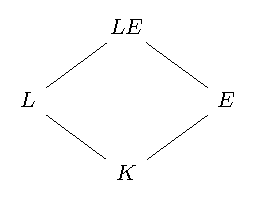
\includegraphics{lectures/5/pictures/pic_4.pdf}
		\end{center}

		Тогда мы имеем
		\[
			e = e\lr*{E/K} = [E : K] \ge [LE : L] \ge e\lr*{LE/L} = e\lr*{LE/K} = e\lr*{E/K} \cdot e\lr*{LE/E}.
		\]
		Отсюда мы получаем, что $e\lr*{LE/E} = 1$, то есть $LE/E$ неразветвлённое. 
	\end{proof}

	\begin{remark}
		Отметим, что так как поля здесь локальные, мы не говорим о сепарабельности (так как конечное расширение кончного поля сепарабельно всегда). 

		Подобные результаты можно получать и не для глобальных полей, но мы этого делать не будем. 
	\end{remark}

	На этом мы прервёмся в изучении локальных полей и перейдём к несколько другой технике, которая нам понадобится для классификации абелевых расширений поля $\Q_{p}$. 

	\subsection{Когомологии групп}

	\noindent\bf{Проективные резольвенты}

	Пусть $G$~--- группа, рассмотрим категорию $G\text{-}\Mod$, (т.е. модулей над групповым кольцом $\Z[G]$). Мы будем рассматривать проективные резольвенты модуля $\Z$ (как $\Z[G]$-модуля с тождественным действием $G$ на $\Z$: $ga = a \ \forall g \in G, a \in \Z$). Для начала давайте построим проективную резольвенту и увидим несколько очевидных свойств. 

	Ясно, что любой модуль можно сюръективно накрыть проективным, сделаем это с $\Z$, т.е. рассмотрим проективный модуль $P_0 \in \Z[G]\text{-}\Mod$:
	\[
		P_0 \overset{\varphi}\twoheadrightarrow \Z \to 0.
	\]

	Теперь мы опять можем сюръективно  накрыть $\ker{\varphi}$ проективным модулем $P_1$ и тогда мы получим точную последоватльность 
	\[
		P_1 \to P_0 \twoheadrightarrow \Z \to 0.
	\]

	Продолжая в том же духе, мы получаем \emph{проективную резольвенту $P_{\bullet}$} $G$-модуля $\Z$:
	\[
		\ldots \to P_2 \to P_1 \xrightarrow{\varphi_1} P_0 \overset{\varphi_0}\twoheadrightarrow \Z \to 0.
	\]

	Ясно, что построение не было ни в коем смысле каноническим и зависело от многих выборов. Кроме того, ясно, что гомологии такого комплекса будут нулевыми просто по определению. 

	Пусть у нас есть две проективные резольвенты $P_{\bullet}$ и $Q_{\bullet}$ модуля $\Z$, построим морфизм $P_{\bullet} \to Q_{\bullet}$:
	\begin{center}
			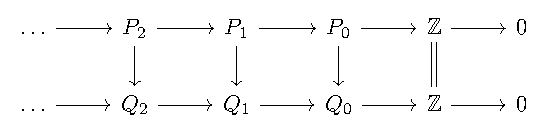
\includegraphics{lectures/5/pictures/pic_5.pdf}
		\end{center}

	Построим сначала отображение $P_0 \to Q_0$. Это можно сделать просто из проективности: 
	\begin{center}
			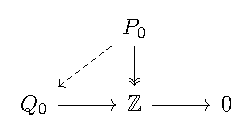
\includegraphics{lectures/5/pictures/pic_6.pdf}
		\end{center}


	Вторую вертикальную стрелку мы строим из двух таких диаграмм:  \textcolor{red}{этого я уже не успел..}


	Остальные будут строятся аналогично. Так мы получаем морфизм комплексов $\alpha\colon P_{\bullet} \to Q_{\bullet}$. Предположим, что у нас есть другой морфизм $\beta\colon P_{\bullet} \to Q_{\bullet}$. Сейчас мы построим цепную гомотопию между $\alpha$ и $\beta$: 

	\begin{center}
		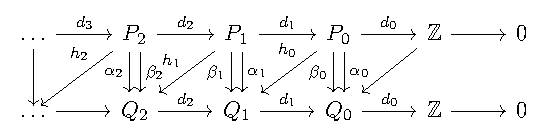
\includegraphics{lectures/5/pictures/pic_9.pdf}
	\end{center}

	Ясно, что мы хотим построить такое отображение $h\colon P_{\bullet} \to Q_{\bullet + 1}$, что 
	\[
		\alpha - \beta = dh + hd.
	\]

	Заметим, что 
	\[
		d_0 \alpha_0 = d_0 = d_0 \beta_0 \implies d_0(\alpha_0 - \beta_0) = 0 \implies \Im{\alpha_0 - \beta_0} \subset \Ker{d_0} = \Im{d_1}.
	\]
	Тогда по проективности мы мозжем замкнуть следующий коммутативный треугольник:
	\begin{center}
			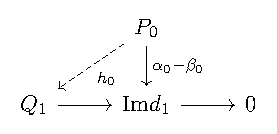
\includegraphics{lectures/5/pictures/pic_7.pdf}
		\end{center}
	и таким образом построить нужное нам отображение $h_0$.  Построим теперь отображение $h_1$. 

	\[
		d_1(\alpha_1 - \beta_1 - h_0 d_1) = d_1(\alpha_1 = \beta_1) + d_1 h_0 d_1 = d_1(\alpha_1 - \beta_1) - (\alpha_0 - \beta_0) d_1 = 0
	\]
	в силу коммутативности диаграммы. Тогда $\alpha_1 - \beta_1 - h_0 d_1 \subset \Ker{d_1} = \Im{d_2}$, откуда мы снова имеем диаграмму: 
	\begin{center}
			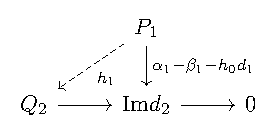
\includegraphics{lectures/5/pictures/pic_8.pdf}
		\end{center}
	и замыкая её по проективности получаем нужное отображение $h_1$. Продолжая в том же духе, мы наконец строим цепную гомотопию $h$. 	

	Теперь рассмотрим проективную резольвенту $P_{\bullet}$ и применим к ней функтор $\Hom(\_, A)$, где $A \in \Z[G]\text{-}\Mod$, тогда мы получим комплекс 
	\[
		 0 \to \Hom_{G}(P_0, A) \to \Hom_{G}(P_1, A) \to \Hom_{G}(P_2, A) \to \ldots
	\]

	\begin{definition} 
		Гомологии построенного выше комплекса 
		\[
			 0 \to \Hom_{G}(P_0, A) \to \Hom_{G}(P_1, A) \to \Hom_{G}(P_2, A) \to \ldots
		\]
		мы будем называть группами \emph{когомологий} группы $G$ с коэффициентами в $\Z[G]$-модуле $A$ и обозначать, как  $H^{i}(G, A)$.
	\end{definition}

	\begin{remark}
		Вообще говоря, пока что наша конструкция зависит от выбора проективной резольвенты (позже мы покажем, что это вообще говоря не так).
	\end{remark}

	Посмотрим сначала на нулевые когомологии. Так как функтор $\Hom(\_, A)$ точен слева, последовательность 
	\[
		0 \to \Hom_{G}(\Z, A) \to \Hom_{G}(P_0, A) \to \Hom(P_1, A)
	\]
	будет точной. В частности, отображение $\Hom_{G}(\Z, A) \to \Hom_{G}(P_0, A)$~--- эпиморфизм. Посмотрим, как устроена группа $\Hom_{G}(\Z, A)$: пусть $n \in \Z, \ \varphi \colon \Z \to A$. Тогда $\varphi(gn) = g \varphi(n) \implies \varphi(n) = g\varphi(n)$, то есть в частности $\varphi(1) = g \varphi(1)$. Так мы получаем, что 

	\[
		\Hom_{G}(\Z, A) \xrightarrow{\sim} A^{G} = \{ a \in A \ \vert \ \forall g \in G \ ga = a \}, \quad \varphi \mapsto \varphi(1) \in A^{G}. 
	\]
	Ясно, что это отображение инъективно (так как $\varphi$ это гомоморфизм групп), покажем сюръектвность. Для $a \in A^{G}$ мы можем положить $\varphi(1) = a$ и продолжить $\varphi$ вполне естественным способом, полагая $\varphi(n) = na$, получая таким образом $\varphi \in \Hom_{G}(\Z, A)$. 

	Таким образом, мы показали, что 
	\[
		H^{0}(G; A) \cong A^{G}.
	\]

	Теперь покажем, что определение когомологий в принципе не зависит от выбора проективной резольвенты. Если у нас есть две проективные резольвенты, то есть и два комплекса: 

	
	\begin{center}
	\centerline{\textcolor{red}{Опять диаграмму для цепной гомотопии так быстро рисовать я её не умею!!!}}
	\end{center}

	\begin{remark}
		\textcolor{red}{Тут нужно переписать пояснения из планшета}.
	\end{remark}

	Итак, мы показали, что когомологии не зависят от выбора проективной резольвенты и таким образом корректно определены. 

	Как и всегда, стандартным образом получается длинная точная последовательность когомологий: 

	\begin{theorem}[Длинная точная последовательность когомологий] 
		Пусть $0 \to A \to B \to C$~--- точная последовательность $G$-модулей. Тогда имеется естественная длинная точная последовательность групп когомологий:
		\begin{multline*}
			0 \to H^{0}(G; A) \to H^{0}(G; B) \to H^{0}(G; C) \to H^{1}(G; A) \to H^{1}(G; B) \to \ldots \to \\ \to H^{n}(G; A) \to H^{n}(G; B) \to H^{n}(G; C) \to H^{n + 1}(G, A) \to \ldots
		\end{multline*}
	\end{theorem}


	\begin{remark}
		Обычно эта теорема применяется таким образом: если мы для некоторого модуля $B$ вдруг знаем, что 
		$H^{n - 1}(B) = H^{n}(B) = 0$, то мы получим кусок 
		\[
			\ldots \to 0 \to H^{n - 1}(G; C) \xrightarrow{\sim} H^{n}(G; A) \to 0 \ldots 
		\]
		и в силу точности мы получим $H^{n - 1}(G; C) \cong H^{n}(G; A)$.
	\end{remark}
 
 	\noindent\bf{Стандартная резольвента}

 	Оказывается, для $\Z$ всегда можно построить \emph{стандартную} проективную резольвенту, состоящую из свободных модулей. А именно, положим $P_i = \Z[G^{i + 1}]$ и рассмотрим 
 	\[
 		\ldots \to \Z[G^3] \xrightarrow{d_2} \Z[G^2] \xrightarrow{d_1} \Z[G] \to \Z
 	\]
 	 $P_i$~--- это свободный $\Z[G]$-модуль, базис которого имеет вид 
 	\[
 		\{ (1, g_1, \ldots, g_{i}) \ \vert \ g_i \in G \}.
 	\]

 		\begin{exercise}
 				Докажите это.  
 			\end{exercise}	
 	Дифференциалы определяются следующим образом: 
 	\[
 		d_i(g_0, \ldots, g_i) = \sum_{j = 0}^{i} (-1)^i (g_0, \ldots, g_{i - 1}, g_{i + 1}, \ldots, g_i), i \ge 1,
	\]		
	а отображение $P_0 \to \Z$ будет просто аугументацией. 

	Для данной резольвенты можно построить цепную гомотопию $h$ между тождественным отображением и нулевым. Она строится следующим образом:
	\[
		h(g_0, \ldots, g_i) = (s, g_0, g_1, \ldots, g_{i}), \quad s \in G
	\]
	и $s$~--- заранее выбранный фиксированный элемент. Тогда мы имеем 
	\[
		dh + hd = \id
	\]

	Отсюда можно вывести точность, а именно, 
	\[
		dh(x) + hd(x) = x \implies (dx = 0 \implies x = dh(x)).
	\]

	Теперь заметим, что $\Hom_{G}(\Z[G^{i + 1}], A)$ состоит просто из функций $f\colon G^{i + 1} \to A$, которые удовлетворяют $f(\sigma g_0, \ldots, \sigma g_n) = \sigma f(g_0, \ldots, g_n)$. Тогда ясно, что $f$ определяется своими значениями на элементах вида $(1, g_1, g_1 g_2, \ldots, g_1 g_2 \ldots g_i)$ и тогда $f$ мы можем интерпретировать её, как функцию 
	\[
		\varphi(g_1, \ldots, g_i) \eqdef f(1, g_1, g_1 g_2, \ldots, g_1 g_2 \ldots g_i).
	\]

		\begin{exercise}
			Докажите, что 
			\[
				\mathrm{d}\varphi(g_1, g_2, \ldots, g_{i + 1}) = g_1 \varphi(g_2, \ldots, g_{i + 1}) + \sum_{j = 1}^{i}(-1)^i \varphi(g_1, g_2, \ldots, g_{j}g_{j + 1}, \ldots) + (-1)^{i + 1}\varphi(g_1, \ldots, g_i).
			\]
		\end{exercise}

	\textcolor{red}{Вот в этом месте я устал писать в техе и пишу на планшете! Всё в тех я перенесу обязательно! Да-да!}	




	

	





	

